\section{創業機會與構想}
\subsection{創業機會}
在台灣,資訊科技領域備受關注。根據110年經濟部智慧學習產業產值調查報告\cite{ref:110產業產值調查報告}中,智慧學習軟體系統的產值為316.3億元,且每年有數百萬名國高中學生參與程式課程\cite{ref:學生數量},形成龐大的市場需求。軟體系統服務在2021年因疫情影響有顯著提升,成長了79.6\%,顯示軟體系統和線上教學是未來的趨勢。

此外,以視訊為主的教材與虛擬教學也成為培訓的主流\cite{ref:企業培訓},MOOCs平台如Udacity、Coursera、Intrepid等,協助Google、Microsoft、AT\&T等大型企業的培訓需求。而在台灣,也有許多教育機構如台灣大學、清華大學、交通大學等,提供具學分、證照、微學位等的線上課程,並有許多學生參與。

\subsection{創業構想}

在面對數位化學習的潮流下,學校、企業、個體教師、補教業者、程式才藝班等族群或機構紛紛加入了線上教學的行列,但是仍然存在著許多挑戰和需求\cite{ref:110產業產值調查報告}\cite{ref:111產業產值調查報告}。例如,數位轉型所具備的技術門檻、教育資源的整合和優化、個性化學習的需求、即時互動的困難與教師教學負擔的增加\cite{ref:老師的困難}等。因此,我們認為在這樣的市場環境下,有機會為客戶提供技術支援或教學工具,以解決這些問題。

\subsection{團隊介紹與歷年得獎}

普羅程式於2021年成立,由四位海大資工系學生組成,成員中有具備全端工程師專業背景與發表AI相關論文於IEEE研討會的成員,並由海大資工的馬尚彬正教授、魚樂天地鄉鎮應援團的何立德執行長分別擔任技術顧問和商業顧問。

團隊成員皆有豐富的程式設計、軟體開發、計畫執行、數位行銷等經驗,並於海大教學中心參與多次創業研習。我們曾在全國性比賽中獲得多項獎項,包括2023資訊智慧創新跨域專題競賽特優獎(圖\ref{fig:Awards-1})並登上年代新聞(圖\ref{fig:News})、2021年潮創客大賽優選獎(圖\ref{fig:Awards-2})、2021武漢金銀湖盃第七屆海峽兩岸青年創新創業大賽入選台灣賽區菁英賽決賽。

\begin{figure}[H]
  \centering
  \begin{subfigure}{0.32\linewidth}
    \centering
    %   \href{https://raw.githubusercontent.com/programingtw/proglearn-plan/main/img/interactiveMeterial.png}{ 
    
\includegraphics[width=0.8\textwidth]{images/年代新聞.jpg}
    %   }
    \caption{年代新聞}
    \label{fig:News}
  \end{subfigure}
    \begin{subfigure}{0.31\linewidth}
    \centering
    %   \href{https://raw.githubusercontent.com/programingtw/proglearn-plan/main/img/interactiveMeterial2.png}{ 
    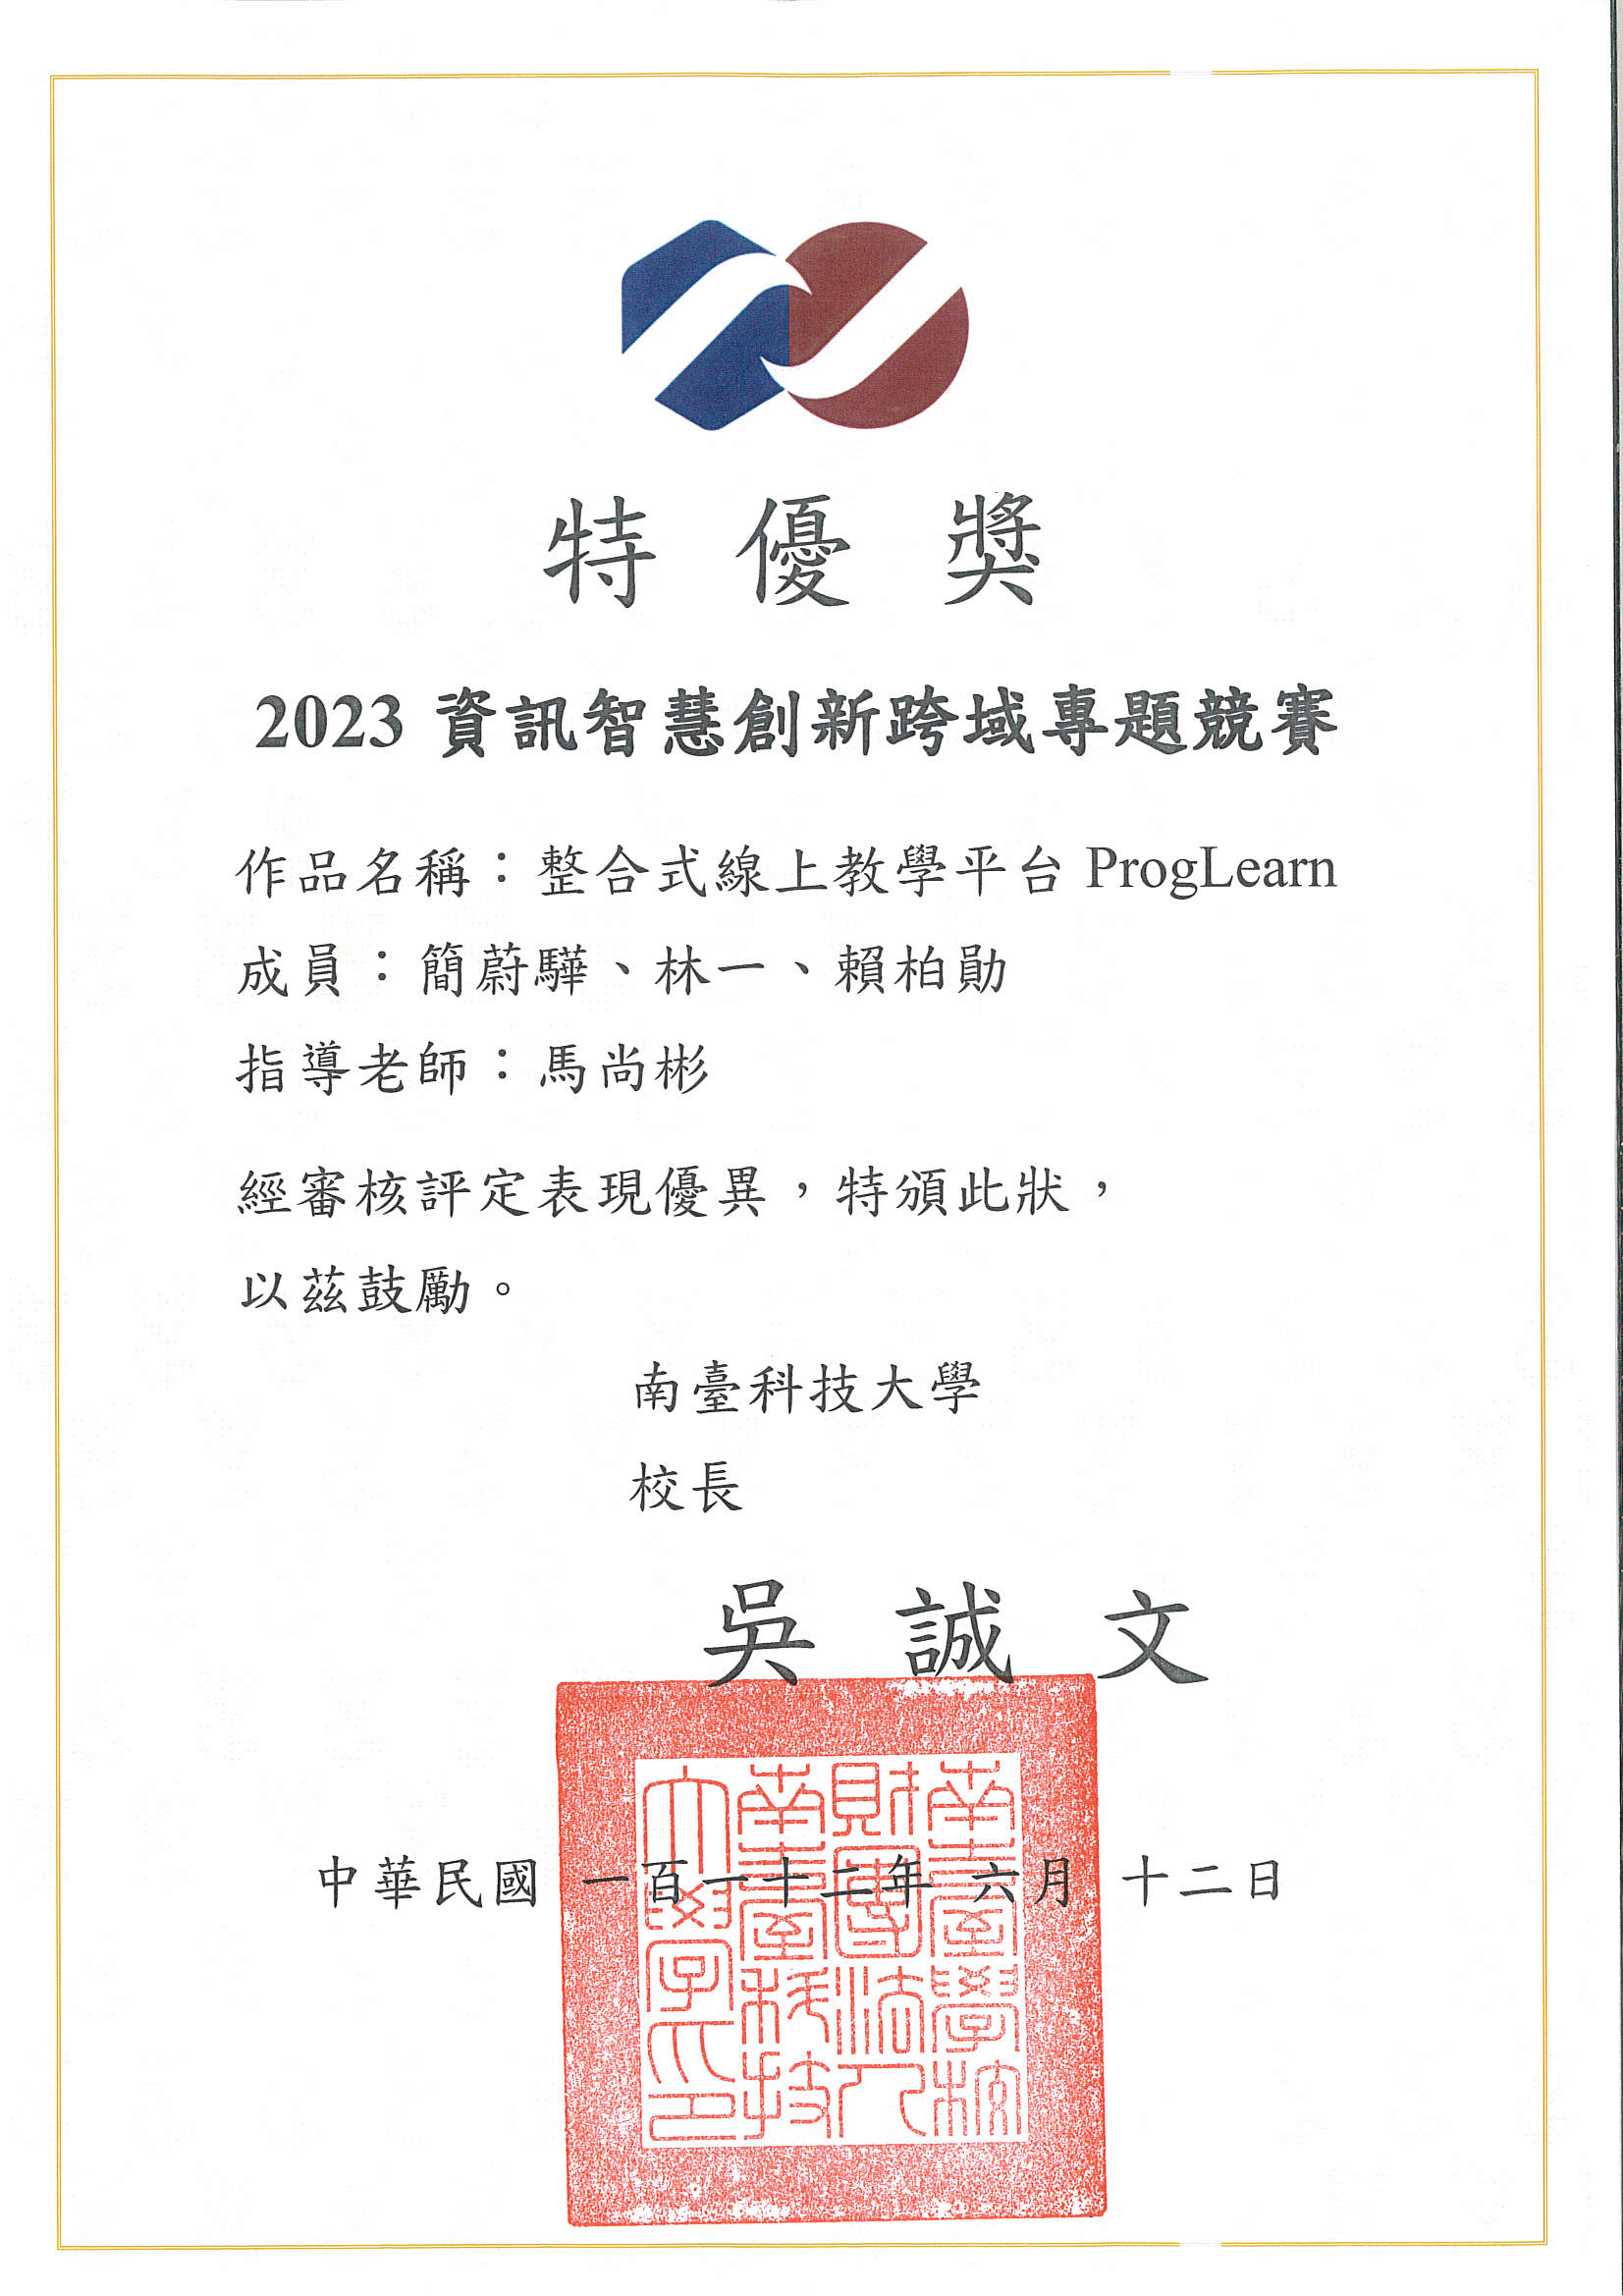
\includegraphics[width=0.45\textwidth]{images/ProgLearn.jpg}
    %   }
    \caption{資訊智慧創新跨域專題競賽}
    \label{fig:Awards-1}
  \end{subfigure}
  \begin{subfigure}{0.31\linewidth}
    \centering
      %   \href{https://raw.githubusercontent.com/programingtw/proglearn-plan/main/img/interactiveMeterial2.png}{ 
    
\includegraphics[width=0.45\textwidth]{images/創博匯.jpg}
      %   }
    \caption{潮創客大賽}
    \label{fig:Awards-2}
  \end{subfigure}
  \caption{團隊榮譽}
\end{figure}